%
%===============>>  Ленотьева Модуль 7 <<=============
%
\setmodule{8}

%BEGIN_FOLD % ====>>_____ Занятие 1 _____<<====
\begin{class}[number=1]
	\begin{listofex}
		\item 
		\begin{minipage}[t]{\bodywidth}
			На клетчатой бумаге с размером клетки 1х1 изображён параллелограмм. Найдите его площадь.
		\end{minipage}
		\hspace{0.02\linewidth}
		\begin{minipage}[t]{\picwidth}
			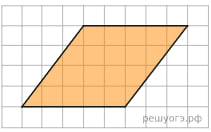
\includegraphics[align=t, width=\linewidth]{../../../../../exercises/lists/pics/leontevaM8L1-1}
		\end{minipage}
		\item 
		\begin{minipage}[t]{\bodywidth}
			На клетчатой бумаге с размером клетки 1х1 изображён параллелограмм. Найдите его площадь.
		\end{minipage}
		\hspace{0.02\linewidth}
		\begin{minipage}[t]{\picwidth}
			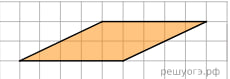
\includegraphics[align=t, width=\linewidth]{../../../../../exercises/lists/pics/leontevaM8L1-2}
		\end{minipage}
		\item Найдите величину острого угла параллелограмма \( ABCD \), если биссектриса угла \( A \) образует со стороной \( BC \) угол, равный \( 43\degree \). Ответ дайте в градусах.
		\item В параллелограмме \( ABCD \) диагональ \( AC \) в \( 2 \) раза больше стороны \( AB \) и \( \angle ACD=111\degree \). Найдите угол между диагоналями параллелограмма. Ответ дайте в градусах.
		\item Диагональ \( BD \)  параллелограмма \( ABCD \)  образует с его сторонами углы, равные \( 50\degree \) и \( 85\degree \). Найдите уголы параллелограмма.
		\item В прямоугольнике диагональ равна \( 10 \), а угол между ней и одной из сторон равен \( 60\degree \), длина этой стороны равна \( 5 \). Найдите площадь прямоугольника, деленную на \( \sqrt{3} \).
		\item В прямоугольнике одна сторона равна \( 96 \), а диагональ равна \( 100 \). Найдите площадь прямоугольника.
		\item Найдите площадь квадрата, если его диагональ равна \( 3 \).
		\item Найдите площадь прямоугольника, если его периметр равен \( 102 \), а отношение соседних сторон равно \(  2:15 \).
		\item На экзамене \( 25 \) билетов, Сергей не выучил \( 3 \) из них. Найдите вероятность того, что ему попадётся выученный билет.
		\item Коля выбирает трехзначное число. Найдите вероятность того, что оно делится на \( 5 \).
		\item Телевизор у Маши сломался и показывает только один случайный канал. Маша включает телевизор. В это время по трем каналам из двадцати показывают кинокомедии. Найдите вероятность того, что Маша попадет на канал, где комедия не идет.
		\item На тарелке \( 12 \) пирожков: \( 5 \) с мясом, \( 4 \) с капустой и \( 3 \) с вишней. Наташа наугад выбирает один пирожок. Найдите вероятность того, что он окажется с вишней.
		\item В каждой десятой банке кофе согласно условиям акции есть приз. Призы распределены по банкам случайно. Варя покупает банку кофе в надежде выиграть приз. Найдите вероятность того, что Варя не найдет приз в своей банке.
		\item В случайном эксперименте симметричную монету бросают дважды. Найдите вероятность того, что орел выпадет ровно \( 1 \) раз.
		\item Игральную кость бросают дважды. Найдите вероятность того, что оба раза выпало число, большее \( 3 \).
		
	\end{listofex}
\end{class}
%END_FOLD

%BEGIN_FOLD % ====>>_____ Занятие 2 _____<<====
\begin{class}[number=2]
	\begin{listofex}
		
		\item Решите уравнение \( x^{2} =2x+8 \).
		\item Найдите корень уравнения \( (x + 10)(- x - 8)=0 \).
		\item Решите уравнение  \( -x^{2}-6x+16=0 \). Если корней больше одного, в ответе укажите бóльший корень.
		\item Решите уравнение: \( \dfrac{5x}{9}=\dfrac{1}{8}:\mfrac{3}{3}{4} \)
		\item 
		\begin{minipage}[t]{\bodywidth}
			На клетчатой бумаге нарисованы два круга. Площадь внутреннего круга равна 15 м. Найдите площадь заштрихованной фигуры. 
		\end{minipage}
		\hspace{0.02\linewidth}
		\begin{minipage}[t]{\picwidth}
			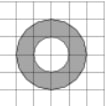
\includegraphics[align=t, width=\linewidth]{../../../../../exercises/lists/pics/leontevaM8L2-3}
		\end{minipage}
		\item \( AC \) и \( BD \)  — диаметры окружности с центром \( O \). Угол \( ACB \) равен \( 55\degree \). Найдите угол \( AOD \). Ответ дайте в градусах.
		\item Центр окружности, описанной около треугольника \( ABC \), лежит на стороне \( AB \). Найдите угол \( ABC \), если угол \( BAC \) равен \( 74\degree \). Ответ дайте в градусах.
		\item Отрезок \( AB  =  8 \) касается окружности радиуса \( 6 \) с центром \( O \) в точке \( B \). Окружность пересекает отрезок \( AO \) в точке \(  D \). Найдите \( AD \).
		\item На окружности по разные стороны от диаметра \( AB \) взяты точки \( M \) и \( N \). Известно, что \( \angle NBA  =  38\degree \). Найдите угол \( NMB \). Ответ дайте в градусах.
		\item Касательные в точках \( A \) и \( B \) к окружности с центром в точке \( O  \) пересекаются под углом \( 82\degree \). Найдите угол \( ABO \). Ответ дайте в градусах.
		\item Отрезки \( AB \) и \( CD \) являются хордами окружности. Найдите длину хорды \( CD \), если \( AB  =  30 \), а расстояния от центра окружности до хорд \( AB \) и \( CD \) равны соответственно \( 20 \) и \( 15 \).
		\item Найдите площадь кругового сектора, если градусная мера его дуги равна 30º, а радиус круга равен 6 см.
		\item Радиус круга равен \( 3 \), а длина ограничивающей его окружности равна \( 6\pi \). Найдите площадь круга. В ответ запишите площадь, деленную на \( \pi \).
		\item Радиус круга равен \( 1 \). Найдите его площадь, деленную на \( \pi \).
		
	\end{listofex}
\end{class}
%END_FOLD

%BEGIN_FOLD % ====>>_ Домашняя работа 1 _<<====
\begin{homework}[number=1]
	\begin{listofex}
		\item Игральную кость бросают дважды. Найдите вероятность того, что сумма двух выпавших чисел равна \( 4 \) или \( 7 \).
		\item В случайном эксперименте симметричную монету бросают четыре раза. Найдите вероятность того, что орел выпадет ровно \( 2 \) раза.
		\item 
		\begin{minipage}[t]{\bodywidth}
			Найдите площадь параллелограмма, изображенного на рисунке.
		\end{minipage}
		\hspace{0.02\linewidth}
		\begin{minipage}[t]{\picwidth}
			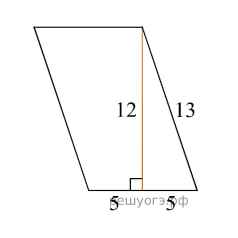
\includegraphics[align=t, width=\linewidth]{../../../../../exercises/lists/pics/leontevaM8L2-1}
		\end{minipage}
		\item В параллелограмме \( ABCD \) диагональ \( AC \) в \( 2 \) раза больше стороны \( AB \) и \( \angle ACD=19\degree \). Найдите угол между диагоналями параллелограмма. Ответ дайте в градусах.
		\item В ромбе \( ABCD \) угол \( ABC \) равен \( 72\degree \). Найдите угол \( ACD \). Ответ дайте в градусах.
		\item Радиус круга равен \( 5 \), а длина ограничивающей его окружности равна \( 6\pi \). Найдите площадь круга. В ответ запишите площадь, деленную на \( \pi \).
		\item Радиус круга равен \( 2 \). Найдите его площадь, деленную на \( \pi \).
	\end{listofex}
\end{homework}
%END_FOLD

%BEGIN_FOLD % ====>>_____ Занятие 3 _____<<====
\begin{class}[number=3]
	\begin{listofex}
		 \item В мешке содержатся жетоны с номерами от \( 5 \) до \( 54 \) включительно. Какова вероятность, того, что извлеченный наугад из мешка жетон содержит двузначное число?
		\item В денежно-вещевой лотерее на \( 100 000 \) билетов разыгрывается \( 1300 \) вещевых и \( 850 \) денежных выигрышей. Какова вероятность получить вещевой выигрыш?
		\item Определите вероятность того, что при бросании игрального кубика (правильной кости) выпадет нечетное число очков.
		
		\item В прямоугольнике одна сторона равна \( 96 \), а диагональ равна \( 100 \). Найдите площадь прямоугольника.
		\item 
		\begin{minipage}[t]{\bodywidth}
			На клетчатой бумаге с размером клетки \( 1x1 \) изображён ромб. Найдите длину его большей диагонали.
		\end{minipage}
		\hspace{0.02\linewidth}
		\begin{minipage}[t]{\picwidth}
			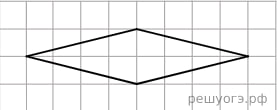
\includegraphics[align=t, width=\linewidth]{../../../../../exercises/lists/pics/leontevaM8L2-2}
		\end{minipage}
		\item Диагонали \( AC \) и \( BD \) параллелограмма \( ABCD \) пересекаются в точке \( O \), \( AC  =  14 \), \( BD  =  18 \), \( AB  =  5 \). Найдите\(  DO \).
		\item Найдите острый угол параллелограмма \( ABCD \), если биссектриса угла \( A \) образует со стороной \( BC \) угол, равный \( 41\degree \). Ответ дайте в градусах.
		\item В параллелограмме \( ABCD \) диагональ \( AC \) в \( 2 \) раза больше стороны \( AB \) и \( \angle ACD=19\degree \). Найдите угол между диагоналями параллелограмма. Ответ дайте в градусах.
		\item В ромбе \( ABCD \) угол \( ABC \) равен \( 72\degree \). Найдите угол \( ACD \). Ответ дайте в градусах.
		\item Площадь ромба равна \( 63 \), а периметр равен \( 36 \). Найдите высоту ромба.
		\item На стороне \( BC \) прямоугольника \( ABCD \), у которого \( AB = 48 \) и \( AD = 112 \), отмечена точка \(  E \) так, что \( \angle EAB = 45\degree \). Найдите \( ED \).
		\item На клетчатой бумаге с размером клетки \( 1 \)см \( × \) \( 1 \)см изображён параллелограмм. Найдите длину его большей высоты. Ответ дайте в сантиметрах. 
	\end{listofex}
\end{class}
%END_FOLD

%BEGIN_FOLD % ====>>_____ Занятие 4 _____<<====
\begin{class}[number=4]
	\begin{listofex}
		\item Занятие 4
	\end{listofex}
\end{class}
%END_FOLD

%BEGIN_FOLD % ====>>_ Домашняя работа 2 _<<====
\begin{homework}[number=2]
	\begin{listofex}
		\item Домашняя работа 2
	\end{listofex}
\end{homework}
%END_FOLD

%BEGIN_FOLD % ====>>_____ Занятие 5 _____<<====
\begin{class}[number=5]
	\begin{listofex}
		\item Занятие 5
	\end{listofex}
\end{class}
%END_FOLD

%BEGIN_FOLD % ====>>_____ Занятие 6 _____<<====
\begin{class}[number=6]
	\begin{listofex}
		\item Занятие 6
	\end{listofex}
\end{class}
%END_FOLD

%BEGIN_FOLD % ====>>_ Домашняя работа 3 _<<====
\begin{homework}[number=3]
	\begin{listofex}
		\item Домашняя работа 3
	\end{listofex}
\end{homework}
%END_FOLD

%BEGIN_FOLD % ====>>_____ Занятие 7 _____<<====
\begin{class}[number=7]
	\title{Подготовка к проверочной}
	\begin{listofex}
		\item Занятие 7
	\end{listofex}
\end{class}
%END_FOLD

=%BEGIN_FOLD % ====>>_ Проверочная работа _<<====
\begin{exam}
	\begin{listofex}
		\item Проверочная
	\end{listofex}
\end{exam}
%END_FOLD